% siminos/spatiotemp/chapter/symFactorXD.tex
% $Author: predrag $ $Date: 2021-07-24 23:53:43 -0400 (Sat, 24 Jul 2021) $

% Xiong 2017-03-08 omitted from the thesis

\section{Discrete factorization of the dynamical zeta function}
\label{sect:fact}

    \PC{2021-06-19}{
    A copy of the 2017-03-09  Xiong Ding's section, not
    included in his thesis\\
    siminos/xiong/thesis/chapters/symFactor.tex.
    }
When a dynamical system has a discrete symmetry, the cycle averaging
formula
% \refeq{eq:sd} and \refeq{eq:zeta}
can be simplified substantially,
and the expansion needs
much fewer orbits to achieve the desired accuracy.
In this section, we discuss how the \dzeta\ can be factorized by a
product of contributions from each irreps of this discrete symmetry.

\subsection{Factorization of $\Cn{3}$ and $\Dn{3}$}

\begin{figure}[h]
  \centering
  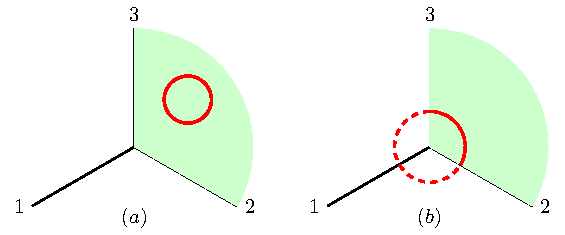
\includegraphics[width=0.9\textwidth]{C3orbits}
  \caption[Orbits in a system with $\Cn{3}$ symmetry.]{
    The two different kinds of \po s in a system with
    $\Cn{3}$ symmetry.
    The green region is the chosen fundamental domain.
    The red cycles are \po s.
  }
  \label{fig:C3orbits}
\end{figure}

$\Cn{3}$ has two subgroups $\{e\}$ and $\{e, \shift, \shift_2\}$, so there
are two types of \po s as shown in \reffig{fig:C3orbits}. A type-(a)
orbit has symmetry $\{e\}$, \ie, no symmetry, and it has two replicas by
rotation $\shift$  and $\shift_2$ respectively, which are not shown in
this figure. So the contribution from
a type-(a) orbit to the \dzeta\
% \refeq{eq:zeta}
is $(1-t_p)^3$.
The cubic order refers to the a fact that there are three sibling orbits together.
Also, since the entire orbit is in the fundamental domain, we have
\[
  1/\zeta_a = (1 - t_{\hat{p}})^3
  \,.
\]
The hat on $p$ means that $t_{\hat{p}}$ is evaluated only on the part of the orbit that
is in the fundamental domain.
A type-(b) orbit is invariant under $e$, $\shift$ and $\shift_2$.
This orbit has no siblings and only one third
of this orbit is in the fundamental domain. The other two thirds are replicas
by rotation $\shift$  and $\shift_2$ of the part in the fundamental domain. So, its
contribution to \dzeta\ is
\[
  1/\zeta_b = 1 - t_p = 1 - t_{\hat{p}}^3
  \,.
\]
Here, relation $t_p= t_{\hat{p}}^3$ is easily obtained by its definition in
\refeq{eq:zeta}.
On the other hand, by \refexam{exam:C3regularRep},
we know that the regular representations of $e$,
$\shift$, and $\shift_2$ are respectively
\[
  D^{reg}(e) = %&=&
  \begin{bmatrix}
    1 & & \\
    & 1 & \\
    & & 1 \\
  \end{bmatrix} \,,  \quad
  % \continue
  D^{reg}(\shift) = %&=&
  \begin{bmatrix}
    ~ & 1 & ~\\
    ~ & ~ & 1\\
    1 & ~ & ~ \\
  \end{bmatrix}\,,  \quad
  D^{reg}(\shift_2) =
  \begin{bmatrix}
    ~ & ~ & 1\\
    1 & ~ & ~\\
    ~ & 1 & ~ \\
  \end{bmatrix}
  \,.
\]
You can easily verify that
\[
 (1 - t_{\hat{p}})^3 = \det(1 - D^{reg}(e)t_{\hat{p}}) \,, \quad
 1 - t_{\hat{p}}^3 = \det(1 - D^{reg}(\shift)t_{\hat{p}}) =
 \det(1 - D^{reg}(\shift_2)t_{\hat{p}})\,.
\]
Therefore, you see that the contribution from \po s to the
\dzeta\ in a system with $\Cn{3}$
symmetry are related to the regular representation of $\Cn{3}$.

\begin{figure}[h]
  \centering
  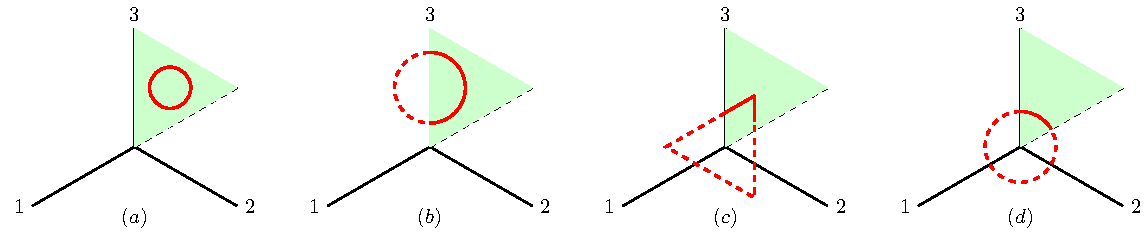
\includegraphics[width=0.9\textwidth]{D3orbits}
  \caption[Orbits in a system with $\Dn{3}$ symmetry.]{
    The four different kinds of \po s in a system with
    $\Dn{3}$ symmetry.
    The green region is the chosen fundamental domain.
    The red cycles are \po s.
  }
  \label{fig:D3orbits}
\end{figure}

Let us check out another example - a system with $\Dn{3}$ symmetry.
$\Dn{3}$ has four different kinds of subgroups $\{e\}$, $\{e, \Refl\}$,
$\{e, \shift, \shift_2\}$, and $\Dn{3}$ itself. Here $\Refl$ can be
any one of $\Refl_{12}$, $\Refl_{23}$ or $\Refl_{31}$. Accordingly,
there are four types of \po s as shown in \reffig{fig:D3orbits}.
The fundamental domain is one sixth of the full \statesp.
Similar to the analysis of the two orbits in the $\Cn{3}$ case, we have
\[
  1/\zeta_a = (1 - t_{\hat{p}})^6
  \,,\quad
  1/\zeta_b = (1 - t_{\hat{p}}^2)^3
  \,,\quad
  1/\zeta_c = (1 - t_{\hat{p}}^3)^2
  \,,\quad
  1/\zeta_d = 1 - t_{\hat{p}}^6
  \,.
\]
\refExam{exam:D3regularRep??} gives the regular representation of $\Dn{3}$.
You can also verify that
\begin{align*}
   & (1 - t_{\hat{p}})^6 = \det(1 - D^{reg}(e)t_{\hat{p}}) \,, \quad
     (1 - t_{\hat{p}}^2)^3 = \det(1 - D^{reg}(\Refl)t_{\hat{p}}) \\
   & (1 - t_{\hat{p}}^3)^2 = \det(1 - D^{reg}(\shift)t_{\hat{p}})\,,\quad
     1 - t_{\hat{p}}^6 = ?
     \,.
\end{align*}
I leave a question mark above since no analogous expression exists for it.
We will come back to it after proving
the identity \refeq{eq:symfac}.

We can generalize the above observation for a system invariant under
a general discrete group
$\Group=\{e, \LieEl_2, \LieEl_3,\cdots, \LieEl_{|\Group|}\}$.
Let $h$ be an element of $\Group$
with order (period) $m$, \ie, $m$ is the smallest positive integer such
that $h^m = e$. Then we have
\begin{equation}
  \label{eq:symfac}
  (1 - t^m)^{\frac{|G|}{m}} = \det(1 - D^{reg}(h)t)
  \,.
\end{equation}
The proof starts from the matrix identity $\ln\det = \tr\ln$, by which we have
\[
  \ln \det(1 - D^{reg}(h)t) = \tr \ln (1 - D^{reg}(h)t)
  = -\sum_{k=1}^\infty \frac{\tr D^{reg}(h^k)t^k}{k}
  \,.
\]
The last identity above comes from the Taylor expansion
$\ln(1-x) = -\sum_{k=1}^\infty \frac{x^k}{k}$.
As we know, the regular representation of
a group element has nonzero trace if and only if this group element is
$e$. So we have,
\[
  \ln \det(1 - D^{reg}(h)t) =  -\sum_{k=1}^\infty \frac{|G|t^{mk}}{mk}
  =  -\frac{|G|}{m}\sum_{k=1}^\infty \frac{t^{mk}}{k}
  = \frac{|G|}{m} \ln (1 - t^m)
  \,.
\]
Therefore, we obtain \refeq{eq:symfac}. This is why we have the observation
in the $\Cn{3}$ and $\Dn{3}$ example. However, for the type-(d) orbit in
\reffig{fig:D3orbits}, the symmetry group of this orbit is
$\{e, \Refl_{12}, \Refl_{32}, \Refl_{13}, \shift, \shift_2\}$. The order of
$\Refl$ is 2 while the order of $\shift$ is 3. The least common multiple is
6. Therefore, the contribution to the \dzeta\ is $(1-t_{\hat{p}}^6)^{1}$ and it
cannot be written as form $\det(1 - D^{reg}(h)t_{\hat{p}})$ with some $h\in G$.

Actually, we can write
\[
  1-t_{\hat{p}}^6 = \det(1 - D^{reg}(\shift)t_{\hat{p}}^2) \,,\quad
  \text{or} \quad
  1-t_{\hat{p}}^6 = \det(1 - D^{reg}(\Refl)t_{\hat{p}}^3)
\]
With $D^{reg}(\shift)$ the $[3\times 3]$ representation of $\shift$ in group $\Cn{3}$
and $ D^{reg}(\Refl)$ the $[2\times 2]$ representation of $\Refl$ in
reflection group $\{e, \Refl\}$. Anyway, for the type-(d) orbit we
have no choice but to give up the regular representation of $\Dn{3}$.

\subsection{Factorization of $C_n$ and $D_n$}

for a discrete symmetry group
$G=\{{ e},{ g}_2,\ldots,{ g}_{|G|}\}$. The orthogonality and completeness
of projection operator
can be easily verified by the orthogonality relation among characters of
irreducible representation. Define $ \cal L_\alpha=P_\alpha \cal L$, then
the trace of {\evOper} $\cal L$ can be decomposed into a sum of
$ \sum_\alpha \tr {\cal L}_\alpha$ because of the completeness of projection
operators.
\Xiong{2014-05-03}{Here the decomposition of trace just relies on the
  completeness of projection operators, we haven't used the commuting
  relation between {\evOper} and group transform. Am I right?}
So we only need to investigate the projected trace formula:
\begin{align*}
  \tr {\cal L}_\alpha & = \frac{d_\alpha}{|G|}\sum_{h \LieEl\in\Group} \chi_\alpha (h)
                        {\bf h}^{-1} \int_\pS dx \, {\cal L} ( x,x) \\
                      & =\frac{d_\alpha}{|G|}\sum_{h \LieEl\in\Group} \chi_\alpha (h) {\bf h}^{-1}
                        \sum_{a \LieEl\in\Group}\int_{\tilde{\pS}} d(a\tilde{x}) \,{\cal L} (a\tilde{x},a\tilde{x})
  \\
                      & =\frac{d_\alpha}{|G|}\sum_{h \LieEl\in\Group} \chi_\alpha (h) {\bf h}^{-1}\,\cdot
                        |G|\int_{\tilde{\pS}} d(\tilde{x}) \,{\cal L} (\tilde{x},\tilde{x}) \\
                      & = d_\alpha \sum_{h \LieEl\in\Group} \chi_\alpha (h) \int_{\tilde{\pS}} d\tilde{x} \,
                        {\cal L} ({\bf h}^{-1} \tilde{x},\tilde{x})
\end{align*}
In the above derivation, we have used the invariance of {\evOper}
under group transform. For a \po\ in the fundamental domain
$\tilde{p}$, we follow the standard argument in Chaosbook and get
\[
  \int_{\tilde{\pS}} d\tilde{x} \, {\cal L} ({\bf h}^{-1} \tilde{x},\tilde{x}) =
  \cl{\tilde{p}} \sum_{r=1}^\infty
    \frac{ e^{r \beta \cdot \Obser_{\tilde{p}}}}
         {|\det \left( {\bf 1}- {\tilde\monodromy}_{\tilde{p}}^r \right)|}
    \delta_{n,\cl{\tilde{p}} r}\delta_{h,h_{\tilde{p}}^r}
  \,;
\]
so, the {\Fd} is
\bea
F(z) &=& \prod_\alpha F_\alpha (z)^{d_\alpha}
\continue   %\,\, , \quad \quad
F_\alpha (z) &=&
{\rm exp}  \left( - {
    \sum_{\tilde{p}} \sum_{r=1}^\infty \frac{1}{r}
    \frac{\chi_\alpha (h_{\tilde{p}}^r)  z^{\cl{\tilde{p}} r}
          e^{r \beta \cdot \Obser_{\tilde{p}}}}
         {|\det \left( {\bf 1}- {\tilde\monodromy}_{\tilde{p}}^r \right)|}
  } \right)
\,\,  ,
\eea
which is discrete factorization for maps. The same method can be applied to
flows with discrete symmetry:
\[
  F_\alpha (z) =
  {\rm exp}  \left( - {
      \sum_{\tilde{p}} \sum_{r=1}^\infty \frac{1}{r}
      \frac{\chi_\alpha (h_{\tilde{p}}^r) e^{r (\beta \cdot \Obser_{\tilde{p}}-sT_{\tilde{p}})}
      }{| \det \left( {\bf 1}- {\tilde\monodromy}_{\tilde{p}}^r \right) | }
    } \right)
\]

Making an approximation
$| \det \left( {\bf 1}- {\tilde\monodromy}_{\tilde{p}}^r \right) | \approx
|\Lambda_{\tilde{p}}|$ where $\Lambda_{\tilde{p}}$ is the product of all
expanding multipliers, we get the factorized zeta function:
\begin{equation}
  F_\alpha (z) =
  {\rm exp}  \left( -
    \sum_{\tilde{p}} \sum_{r=1}^\infty \frac{1}{r}
    \chi_\alpha (h_{\tilde{p}}^r) t_{\tilde{p}}^r \right)
  \label{eq:redzeta}
\end{equation}

Formula \eqref{eq:redzeta} is the ultimate goal of Discrete Factorization,
which basically tells us that,
equipped with character table of the group in question, we can write down
all the factorized zeta function for all classes of this group. On the
other hand, in order to verify our result,
let's calculate the zeta
function in the full \statesp.
\begin{align*}
  F(z) &= \prod_\alpha F_\alpha (z)^{d_\alpha} \\
       &= {\rm exp}  \left( -
         \sum_{\tilde{p}} \sum_{r=1}^\infty \frac{1}{r}\sum_{\alpha}
         \left(d_{\alpha}\chi_\alpha (h_{\tilde{p}}^r)\right) t_{\tilde{p}}^r \right) \\
       &= {\rm exp}  \left( -
         \sum_{\tilde{p}} \sum_{r=1}^\infty \frac{1}{r}
         |G|\delta_{h_{\tilde{p}}^r}  t_{\tilde{p}}^r \right) \\
       &= {\rm exp}  \left( -
         \sum_{\tilde{p}} \sum_{k=1}^\infty \frac{|G|}{mk}
         t_{\tilde{p}}^{mk} \right)
         \,,
\end{align*}
that is
\begin{equation}
  \label{eq:fullzeta}
  F(z)= \left(1-t_{\tilde{p}}^{\frac{|G|}{m}}\right)^{m} \,,
\end{equation}
where $m$ is the smallest positive number such that $h_{\tilde{p}}^{m}=e$, namely
the multiplicity of the \po\ in the full \statesp.
Formula \eqref{eq:fullzeta} is just the left side of
\beq
(1-t_{\tilde{p}}^{h_p})^{g/h_p}
=\det \left(1- D(h_{\tilde p}) t_{\tilde p} \right)
=
\prod_{\alpha} \det(1-D_{\alpha}(h_{\tilde{p}}) t_{\tilde{p}} )^{d_\alpha}
\eeq
in Chaosbook and actually formula \eqref{eq:redzeta} is the right side of
it. For completeness, I derive their equivalence here. By the
definition of character and representation of a group,
$\chi_\alpha (h_{\tilde{p}}^r)= \tr D_{\alpha}(h_{\tilde{p}}^r)
=\tr (D_{\alpha}(h_{\tilde{p}}))^r$ where $D$ is the regular representation
of this group, so \eqref{eq:redzeta} can be rewritten as follows,
\begin{align*}
  F_\alpha (z) & =
                 {\rm exp}  \left( -
                 \tr \sum_{\tilde{p}} \sum_{r=1}^\infty \frac{1}{r}
                 (D_{\alpha}(h_{\tilde{p}}))^r t_{\tilde{p}}^r \right) \\
               & ={\rm exp}  \left(
                 \tr \sum_{\tilde{p}} \ln (1-D_{\alpha}(h_{\tilde{p}}))
                 \right) \\
               & = \prod_{\tilde{p}} \det(1-D_{\alpha}(h_{\tilde{p}}))
\end{align*}
Here, we have used relation $\tr \ln= \ln \det$. All calculation of
factorized zeta function in Chaosbook is conducted by
$\det(1-D_{\alpha}(h_{\tilde{p}}))$, but I are apt to use \eqref{eq:redzeta}
because it doesn't contain information about any specific representation.
\Xiong{2014-05-05}{I am not sure whether I understand it correctly here.}
All the following examples are analyzed by \eqref{eq:redzeta}.

\paragraph{$C_{n}$} case

When $h_{\tilde p}=e$,
\[
  F_{A}=F_{\Gamma_j}={\rm exp} (-\sum_{r=1}^\infty \frac{1}{r}t_{\tilde{p}}^r )
  =1-t_{\tilde p}
  \,,
\]
Where we only investigate the contribution from one specific periodic
orbit and ignore the summation $ \sum_{\tilde{p}}$.

When $h_{\tilde p}=C_n^k$, Similarly,
\[
  F_{A}=1-t_{\tilde p}
\]
\[
  F_{\Gamma_j}={\rm exp} (-\sum_{r=1}^\infty \frac{1}{r}e^{\frac{i2\pi kjr}{n}}
  t_{\tilde{p}}^r )
  =1-e^{\frac{i2\pi kj}{n}} t_{\tilde p}
  \,,
\]
In sum,
\vskip 12pt
\begin{tabular}{rlccc}

  $h_{\tilde p}$ &  & &  $A$  &  $\Gamma_{j}$ \\
  $e$:
                 & $(1-t_{\tilde p} )^n$  &=&$(1-t_{\tilde p})$ & $(1-t_{\tilde p})$  \\
  $C_n^{k}$:
                 & $(1-t_{\tilde p}^m )^{\frac{n}{n}}$ &=&  $(1-t_{\tilde p})$ & $(1-\exp(\frac{i2\pi kj}{n})t_{\tilde p})$ \\
\end{tabular}
\vskip 12pt
\noindent


\paragraph{$D_{n}$ ($n$ odd)} case:
When $h_{\tilde p}=e$,
\[
  F_{A_1}=F_{A_2}={\rm exp} (-\sum_{r=1}^\infty \frac{1}{r}t_{\tilde{p}}^r )
  =1-t_{\tilde p}
\]
\[
  F_{E_j}={\rm exp} (-\sum_{r=1}^\infty \frac{2}{r}t_{\tilde{p}}^r )
  =(1-t_{\tilde p})^2
\]
When $h_{\tilde p}=C_n^k$, the same goes for $A_1$ and $A_2$:
$F_{A_1}=F_{A_2}=1-t_{\tilde p}$, but for $E_j$, it requires a little
special treatment.
\begin{align*}
  F_{E_j}= & {\rm exp} (-\sum_{r=1}^\infty \frac{1}{r}2\cos\frac{2\pi kjr}{n}
             t_{\tilde{p}}^r ) \\
  = & {\rm exp} \left(-\sum_{r=1}^\infty \frac{1}{r}(\exp(\frac{i2\pi
      kjr}{n})+\exp(-\frac{i2\pi kjr}{n}))t_{\tilde{p}}^r \right) \\
  = & \left(1-\exp(\frac{i2\pi kj}{n})t_{\tilde p} \right)
      \left(1-\exp(-\frac{i2\pi kj}{n})t_{\tilde p} \right) \\
  = & 1-2\cos\frac{2\pi kj}{n}t_{\tilde p}+t_{\tilde p}^2
\end{align*}
When $h_{\tilde p}\in \{\Refl,\Refl_{1},\cdots,\Refl_{n-1}\}$,
$h_{\tilde p}^2=e$.
\begin{align*}
  F_{A_1}= &1-t_{\tilde p} \\
  F_{A_2}= &{\rm exp} (-\sum_{r=even}^\infty \frac{1}{r}t_{\tilde{p}}^r
             +\sum_{r=odd}^\infty \frac{1}{r}t_{\tilde{p}}^r )
             =(1+t_{\tilde p}) \\
  F_{E_j}= &{\rm exp} (-\sum_{r=even}^\infty \frac{1}{r}2t_{\tilde{p}}^r)
             =(1-t_{\tilde p}^2)
\end{align*}

In sum,

\vskip 12pt
\begin{tabular}{rlcccc}

  $h_{\tilde p}$ &  & &  $A_1$  &  $A_2$  &  $E_j$  \\
  $e$:
                 & $(1-t_{\tilde p} )^{2n}$  &=&$(1-t_{\tilde p})$ & $(1-t_{\tilde p})$ &
                                                                                          $ (1-t_{\tilde p})^4 $ \\
  $C_n^k,C_n^{n-k} $:
                 & $(1-t_{\tilde p}^m )^{\frac{2n}{m}}$ &=&  $(1-t_{\tilde p})$ & $(1-t_{\tilde p})$ &
                                                                                                       $ (1-2\cos(\frac{2\pi kj}{n})t_{\tilde p}+t^{2}_{\tilde p})^2 $ \\
  $\Refl,\Refl_{1},\cdots,\Refl_{n-1}$:
                 & $(1-t_{\tilde p}^2 )^{n}$ &=&  $(1-t_{\tilde p})$ &                      $(1+t_{\tilde p})$ &$ (1-t_{\tilde p}^2)^2 $ \\
\end{tabular}
\vskip 12pt
\noindent


\paragraph{$\Dn{n}$ ($n$ even)} case:
% When $h_{\tilde p}=e$, we have $F_{A_1}= %F_{A_2}=F_{B_1}=F_{B_2}=1-t_{\tilde p}$
% and $F_{E_j}=(1-t_{\tilde p})^2$
%
% When $h_{\tilde p}=C_2$, similarly, $F_{A_1}= F_{A_2}=1-t_{\tilde p}$,
% $F_{B_1}=F_{B_2}=1-(-1)^{n/2}t_{\tilde p}$ and
% $F_{E_j}=(1-(-1)^jt_{\tilde p})^2$.

Similar calculation gives us the following
factorized zeta function table.

\vskip 12pt
\begin{center}
  \begin{tabular}{b{1cm}lcccccl}

    $h_{\tilde p}$ &  & &  $A_1$  &  $A_2$  &  $B_1$  &  $B_2$  &  $E_{j}$  \\
    $e$:
                   & $(1-t_{\tilde p} )^{2n}$  &=&$(1-t_{\tilde p})$ & $(1-t_{\tilde p})$ &
                                                                                            $(1-t_{\tilde p})$ &$(1-t_{\tilde p})$&$ (1-t_{\tilde
                                                                                                                                    p})^4 $ \\
    $\shift_{n/2}$:
                   & $(1-t_{\tilde p}^2 )^n$ &=&  $(1-t_{\tilde p})$ & $(1-t_{\tilde p})$ &
                                                                                            $(1-(-1)^{\frac{n}{2}}t_{\tilde p})$ &$(1-(-1)^{\frac{n}{2}}t_{\tilde p})$ &
                                                                                                                                                                         $(1-(-1)^jt_{\tilde p})^4 $ \\
    $\shift_{k}$ (odd):
                   & $(1-t_{\tilde p}^m )^{\frac{2n}{m}}$ &=&  $(1-t_{\tilde p})$ & $(1-t_{\tilde p})$ &
                                                                                                         $(1+t_{\tilde p})$ &$(1+t_{\tilde p})$ &
                                                                                                                                                  $ (1-2\cos(\frac{2\pi kj}{n})t_{\tilde p}+t^{2}_{\tilde p})^2 $ \\
    $\shift_{k}$ (even):
                   & $(1-t_{\tilde p}^m )^{\frac{2n}{m}}$ &=&  $(1-t_{\tilde p})$ & $(1-t_{\tilde p})$ &
                                                                                                         $(1-t_{\tilde p})$ &$(1-t_{\tilde p})$ &
                                                                                                                                                  $ (1-2\cos(\frac{2\pi kj}{n})t_{\tilde p}+t^{2}_{\tilde p})^2 $ \\
    $\Refl$:
                   & $(1-t_{\tilde p}^2 )^n$&=& $(1-t_{\tilde p})$ & $(1+t_{\tilde p})$ &
                                                                                          $(1-t_{\tilde p})$ &$(1+t_{\tilde p})$& $ (1-t_{\tilde p}^2)^2 $ \\
    $\shift\Refl$:
                   & $(1-t_{\tilde p}^2 )^n$&=& $(1-t_{\tilde p})$ & $(1+t_{\tilde p})$ &
                                                                                          $(1+t_{\tilde p})$ &$(1-t_{\tilde p})$& $ (1-t_{\tilde p}^2)^2 $ \\
  \end{tabular}
\end{center}
\vskip 12pt
\noindent

When it comes to continuous symmetry, projection operator is
\beq
{P}_\eigenvG
= d_\eigenvG \int_{G} dg\,
\, \chi_\eigenvG(g^{-1})  O_g
\,.
\eeq
The corresponding trace formula in the irreducible subspace is
\beq
\sum_{\beta=0}^\infty
    \frac{1}{\eigenvL -\eigenvL_{\eigenvG,\beta} }
=
d_\eigenvG \sum_p
\period{p}
\sum_{r=1}^\infty
\chi_\eigenvG( g_p^r)
\frac{e^{r (\beta \Obser_p -\eigenvL\period{p})}}
     {{\left|\det\!\left(\matId-
        \tilde{\monodromy}_{\eigenvG,p}^r\right)\right|}}
\,.
\eeq
Therefore the \Fd\ is factorized as

\bea
\det(\eigenvL - \Aop) &=& \prod_\alpha F_\alpha (z)^{d_\alpha}
\continue   %\,\, , \quad \quad
F_\alpha (z) &=&
{\rm exp}  \left(
    - {
    \sum_{\tilde{p}} \sum_{r=1}^\infty \frac{1}{r}
    \frac{\chi_\alpha (g_{\tilde{p}}^r)  z^{\cl{\tilde{p}} r}
      e^{r \beta \cdot \Obser_{\tilde{p}}}
      % {\phi_p^r}
      } {| \det \left( {\bf 1}- {\tilde\monodromy}_{\tilde{p}}^r \right) | }
       } \right)
\,\,
\eea
It differs from the discrete case on that now the group operator
$g_{\tilde{p}}$ is continuous and the factorization may have infinite terms.

\paragraph{Used formulas} Here I list several formulas used in the
above post.

\begin{equation}
  \frac{1}{2\pi}\sum_{n=-\infty}^{\infty}e^{inx} = \delta(x)
\end{equation}
This identity comes from one definition of delta function
$\delta(x)=\lim_{N\to \infty}
\frac{1}{2\pi}\frac{\sin(N+1/2)x}{\sin(\frac{1}{2}x)}$ and simple
calculation gives
$\sum_{n=-N}^{N}e^{inx}=\frac{\sin(N+1/2)x}{\sin(\frac{1}{2}x)}$.

\begin{equation}
  \sum_{R}\chi_\alpha(R) \chi_\beta(SR^{-1})=\frac{|G|}{d_\alpha}\,
  \delta _{\alpha,\beta} \chi_\alpha(S)
\end{equation}
This is the orthogonality between characters of irreducible
representations. If we set $S=e$, then it reduces to
$\sum_{R}\chi_\alpha(R) \chi_\beta(R^{-1})=|G|\delta _{\alpha,\beta}$.
The orthogonality of projection operators can be checked:
\begin{align*}
  P_\alpha P_\beta = & \frac{d_\alpha}{|G|}\, \frac{d_\beta}{|G|}
                       \sum_{h,s\LieEl\in\Group} \chi_\alpha (h) \chi_\alpha (s) {\bf h}^{-1} {\bf s}^{-1} \\
  = & \frac{d_\alpha}{|G|}\, \frac{d_\beta}{|G|} \sum_{s\LieEl\in\Group}
      \frac{|G|}{d_\alpha}\,\delta _{\alpha,\beta} \chi_\alpha(sh)(\bf{sh})^{-1} \\
  = &\delta _{\alpha,\beta} \frac{d_\alpha}{|G|}\,\sum_{s\LieEl\in\Group}
      \chi_\alpha(s){\bf s}^{-1} \\
  = & \delta _{\alpha,\beta}\, P_\alpha
\end{align*}

The last formula is
\begin{equation}
  \sum_\alpha d_\alpha \chi_\alpha (R) = |G|\, \delta_{e,R}
  \label{eq:groupcomplete}
\end{equation}
which comes from orthogonality relation above. For regular representation,
the trace of $R$ in terms of irreducible representations is
$\chi (R)=\sum_\alpha a_\alpha \chi_\alpha (R)$, so the summation of all group
elements gives
\[
  \sum_{R}\chi (R)\chi_\alpha (R^{-1})=\sum_\alpha a_\alpha \sum_{R}
  \chi_\alpha (R) \chi_\alpha (R^{-1}) =|G|\, a_\alpha
\]
On the other hand, $\chi (R)=|G|\, \delta_{e,R}$ for regular representation,
then the left side of the above expression is just $|G|\,\chi_\alpha (e)$,
so $a_\alpha =\chi_\alpha (e) =d_\alpha $ the dimension of $\alpha_{th}$
irreducible representation. In this way, we obtain \refeq{eq:groupcomplete}.
Now the completeness of projection operator can be checked:
\[
  \sum_\alpha P_\alpha = \sum_\alpha \frac{d_\alpha}{|G|} \sum_{h\LieEl\in\Group}
  \chi_\alpha (h)  {\bf h}^{-1}
  =\frac{1}{|G|} \sum_{h\LieEl\in\Group} \left(\sum_\alpha d_\alpha \chi_\alpha (h)
  \right){\bf h}^{-1}
  =e
\]
